\section{Sample Time}
A bottleneck on the accuracy of the final image is the amount of error introduced by the sampling of the velocity profile produced by the solution of the time-optimal control problem. Sampling error is an unavoidable result of a digital system following a given profile. Thus there is a limit on the accuracy of a digital system, especially one which uses integration in order to achieve an outcome. The smallest amount of error will magnify until the result is quite different from that which is desired. Since a digital processing device can only direct an integrating process at a limited rate, sampling errors will accumulate over time and cause the image to become inaccurate. In the case of the DoodleBot, the measured placement of the initial position at the initialisation of a trajectory resets the integration error and as such the error can only accumulate over a single curve. The effect of operating at differing sample periods can be seen in Figure \ref{fig:timestep}.

\begin{figure}[htbp]  
\includegraphics[width=\textwidth]{figures/performance/timestep.png}
\caption[Comparison of differing velocity sampling frequencies]{A comparison of velocity sampling periods. From top left to bottom right; 1) 20ms 2) 40ms 3) 80ms 4) 120ms 5) 150ms 6) 200ms
\label{fig:timestep}}
\end{figure}  

Two effects are at play in the alteration of the sampling period. A limit exists on the lowering of the sampling period below the time required for the controller to undergo one iteration of the control loop. Beyond this point variance in the loop timing can weight some commands noticeably more than others, even to the point where commands begin to get skipped or are not active for a long enough duration to have an effect. This causes the type of distortion in the final image that can be seen in the top left profile in Figure \ref{fig:timestep}. The second effect of the sampling period on the accuracy of the output image is that an increase in the sampling period corresponds to a larger approximation of the correct velocity profile. The looser an approximation becomes, the greater the integral error will become over the length of the curve. Figure \ref{fig:timestep} demonstrates this effect. As the as the sampling period increases the amount of error becomes progressively greater. Figure \ref{fig:tStep} demonstrates that the level of error in the final image is linearly correlated with respect to the sampling period.
\begin{figure}[htbp]  
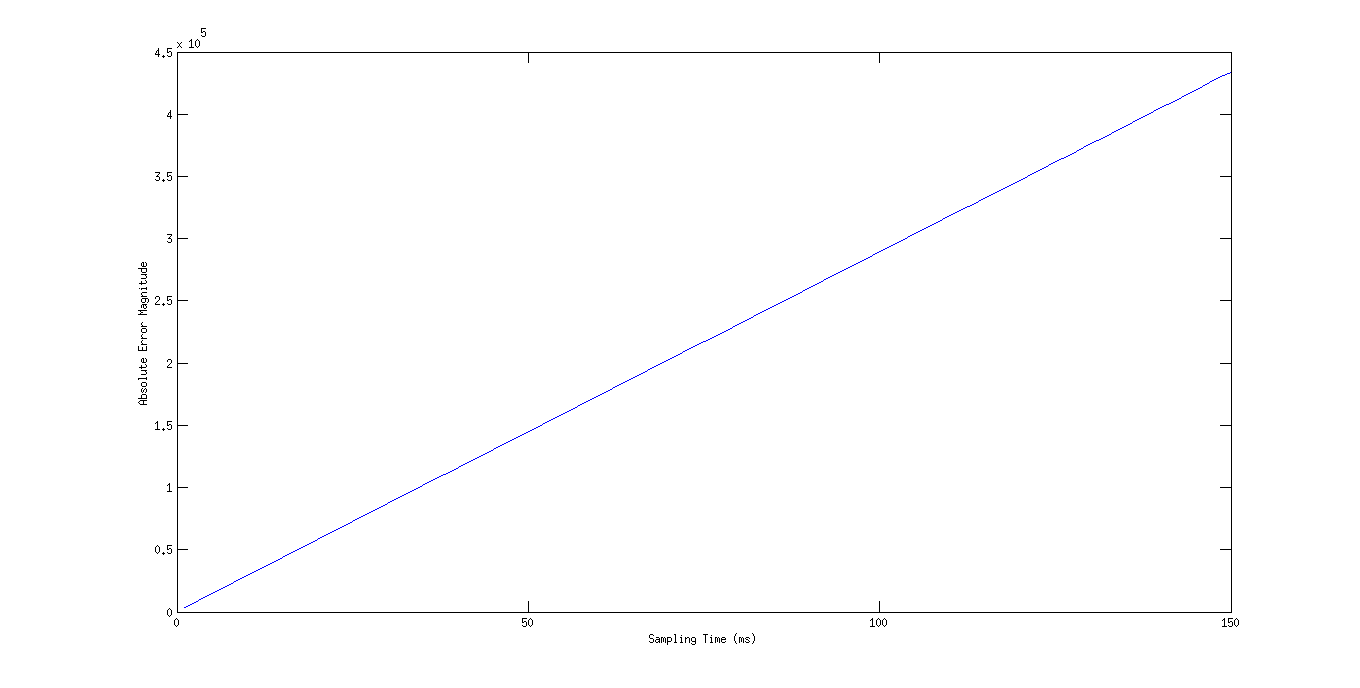
\includegraphics[width=\textwidth]{figures/performance/tStep.png}
\caption[Plot of error magnitude against velocity sampling period]{Error magnitude against velocity sampling period
\label{fig:tStep}}
\end{figure}  
It is evident that the best policy is to decrease the sample period until just before the limits of the control loop manifest. The DoodleBot was found to perform best at a 40ms sampling period, or at 25Hz.